% !TEX TS-program = XeLaTeX
% use the following command: 
% all document files must be coded in UTF-8
\documentclass{textolivre}
% for anonymous submission
%\documentclass[anonymous]{textolivre}
% to create HTML use 
%\documentclass{textolivre-html}
% See more information on the repository: https://github.com/leolca/textolivre

% Metadata
\begin{filecontents*}[overwrite]{article.xmpdata}
    \Title{Desenvolvimento de um corretor ortográfico}
    \Author{Leonardo Carneiro de Araújo \sep Aline de Lima Benevides \sep João Pedro Hallack Sansão}
    \Language{pt-BR}
    \Keywords{corretor ortográfico \sep ortografia \sep afixos \sep linguística computacional}
    \Journaltitle{Texto Livre}
    \Journalnumber{1983-3652}
    \Volume{14}
    \Issue{1}
    \Firstpage{1}
    \Lastpage{19}
    \Doi{10.35699/1983-3652.2021.26469}

    \setRGBcolorprofile{sRGB_IEC61966-2-1_black_scaled.icc}
            {sRGB_IEC61966-2-1_black_scaled}
            {sRGB IEC61966 v2.1 with black scaling}
            {http://www.color.org}
\end{filecontents*}

% used in this example to provide source code environment
\crefname{lstlisting}{lista}{listas}
\Crefname{lstlisting}{Lista}{Listas}
\usepackage{listings}
\renewcommand\lstlistingname{Lista}
\lstset{language=bash,
	breaklines=true,
	basicstyle=\linespread{1}\small\ttfamily,
	numbers=none,xleftmargin=0.5cm,
	frame=none,
	framexleftmargin=0.5em,
	framexrightmargin=0.5em,
	showstringspaces=false,
	upquote=true,
	commentstyle=\color{gray},
	literate=%
           {á}{{\'a}}1 {é}{{\'e}}1 {í}{{\'i}}1 {ó}{{\'o}}1 {ú}{{\'u}}1 
	   {à}{{\`a}}1 {è}{{\`e}}1 {ì}{{\`i}}1 {ò}{{\`o}}1 {ù}{{\`u}}1
           {ã}{{\~a}}1 {ẽ}{{\~e}}1 {ĩ}{{\~i}}1 {õ}{{\~o}}1 {ũ}{{\~u}}1
           {â}{{\^a}}1 {ê}{{\^e}}1 {î}{{\^i}}1 {ô}{{\^o}}1 {û}{{\^u}}1
	   {ä}{{\"a}}1 {ë}{{\"e}}1 {ï}{{\"i}}1 {ö}{{\"o}}1 {ü}{{\"u}}1
	   {Á}{{\'A}}1 {É}{{\'E}}1 {Í}{{\'I}}1 {Ó}{{\'O}}1 {Ú}{{\'U}}1
	   {À}{{\`A}}1 {È}{{\`E}}1 {Ì}{{\`I}}1 {Ò}{{\`O}}1 {Ù}{{\`U}}1
	   {Ã}{{\~A}}1 {Ẽ}{{\~E}}1 {Ũ}{{\~u}}1 {Õ}{{\~O}}1 {Ũ}{{\~U}}1
	   {Â}{{\^A}}1 {Ê}{{\^E}}1 {Î}{{\^I}}1 {Ô}{{\^O}}1 {Û}{{\^U}}1
	   {Ä}{{\"A}}1 {Ë}{{\"E}}1 {Ï}{{\"I}}1 {Ö}{{\"O}}1 {Ü}{{\"U}}1
           {ç}{{\c{c}}}1 {Ç}{{\c{C}}}1
}

\journalname{Texto Livre: Linguagem e Tecnologia}
\thevolume{14}
\thenumber{1}
\theyear{2021}
\receiveddate{\DTMdisplaydate{2020}{11}{27}{-1}} % YYYY MM DD
\accepteddate{\DTMdisplaydate{2021}{1}{4}{-1}}
\publisheddate{\DTMdisplaydate{2021}{2}{09}{-1}}
% Corresponding author
\corrauthor{Leonardo Araújo}
% DOI
\articledoi{10.35699/1983-3652.2021.26469}
% list of available sesscions in the journal: articles, dossier, reports, essays, reviews, interviews, editorial
\articlesessionname{Linguística e Tecnologia}
% Abbreviated author list for the running footer
\runningauthor{Araújo et al.}

\title{Desenvolvimento de um corretor ortográfico}
\othertitle{Developing a spell checker}
% if there is a third language title, add here:
%\othertitle{Artikelvorlage zur Einreichung beim Texto Livre Journal}

\author[1]{Leonardo Carneiro de Araújo \orcid{0000-0003-3884-2177} \thanks{Email: \url{leolca@ufsj.edu.br}}}
\author[2]{Aline de Lima Benevides \orcid{0000-0003-1814-593X} \thanks{Email: \url{benevides.aline12@gmail.com}}}
\author[1]{João Pedro H. Sansão \orcid{0000-0003-0095-2629} \thanks{Email: \url{joao@ufsj.edu.br}}}

\affil[1]{Universidade Federal de São João del Rei, Brasil.}
\affil[2]{Universidade de São Paulo, Brasil.}

% Corresponding author
\corrauthor{Leonardo Araújo}
% DOI
\articledoi{10.35699/1983-3652.2021.26469}
% Abbreviated author list for the running footer
\runningauthor{Araújo et al.}
\editorname{Daniervelin Pereira}

%\usepackage[backend=biber,style=abnt, ittitles]{biblatex}
%\DeclareLanguageMapping{brazil}{brazil-apa}
\addbibresource{article.bib}     
% use biber instead of bibtex
% $ biber tl-article-template
% $ pdflatex tl-article-template.tex

% set language of the article
\setdefaultlanguage[variant=brazilian]{portuguese}
\setotherlanguage{english}
% for langues that use special fonts, you must provide the typeface that will be used
% \setotherlanguage{arabic}
% \newfontfamily\arabicfont[Script=Arabic]{Amiri}
% \newfontfamily\arabicfontsf[Script=Arabic]{Amiri}
% \newfontfamily\arabicfonttt[Script=Arabic]{Amiri}
%
% in the article, to add arabic text use: \textlang{arabic}{ ... }


\usepackage{multirow}
%\usepackage{sansmath}
%\sansmath

%\usepackage{sfmath}
%\usepackage{cmbright}

\begin{document}
\maketitle

\begin{polyabstract}
\begin{abstract}
Corretores ortográficos são ferramentas computacionais utilizadas cotidianamente
na redação de textos e de mensagens ou, de forma oculta, na busca por informação e mineração
de dados. Diante de sua relevância, o presente trabalho apresenta
o percurso histórico de desenvolvimento dos corretores ortográficos
e ilustra como, 
de forma simples, é possível criar um corretor ortográfico eficiente a partir
da proposta de \textcite{norvig2007}.
Salientam-se, também, algumas ferramentas e as estratégias empregadas na elaboração
de corretores, como a remoção de afixos e a computação de n-gramas.
Explicita-se, ainda, a implementação do corretor ortográfico de \textcite{norvig2007} e
verifica-se seu desempenho na tarefa de correção automática em diferentes conjuntos de
dados de erros ortográficos. Expõe-se, também, uma comparação na performance de um corretor ortográfico
que se vale da remoção de afixos em relação a um corretor que não adota semelhante estratégia.

\keywords{corretor ortográfico \sep ortografia \sep afixos \sep linguística computacional}
\end{abstract}

\begin{english}
\begin{abstract}
Spell checkers are ubiquitous computational tools that help us in correctly writing texts or messages
and improving information inquiry and data mining.
The present work presents the history of development of spell checkers and illustrates how,
in a simple way, it is possible to create an efficient spell checker from Norvig's proposal. % of \textcite{norvig2007}.
We also highlight some tools and how they are used in the development of spell checkers, such as affix removal and n-gram computation.
Moreover, we present an implementation of Norvig's spell checker and its performance
in automatic correction for different spelling error data sets.
Also, in a comparison of spell checkers performance, we expose that it is worth removing affixes.

\keywords{spell checker \sep spelling \sep orthography \sep affixes \sep computational linguistics}
\end{abstract}
\end{english}

% if there is another abstract, insert it here using the same scheme
\end{polyabstract}



\section{Introdução}\label{sec-intro}

Corretores ortográficos são ferramentas conhecidas por usuários de computadores ou de celulares 
por terem um papel importante na elaboração de textos. Eles são utilizados para detectar erros 
ortográficos e sugerir correções - palavras ortográficas semelhantes à palavra escrita pelo usuário, 
que provavelmente corresponde àquela pretendida por quem escreve, sem qualquer erro ortográfico. 
Ainda que esta seja a sua função mais popular, sua utilidade vai além da mera sugestão de palavras. 
A tarefa de um corretor ortográfico é, primariamente, o reconhecimento e a classificação de padrões. 
Eles são muito úteis em tarefas de recuperação de informação e em ferramentas de busca \cite{brill2005,shazeer2007,cameron2013}, uma vez que 
tanto a pergunta de um usuário quanto a informação armazenada podem estar grafadas de maneira diversa 
da sequência grafêmica da palavra alvo,
sendo necessário encontrar padrões que as aproximem, sem a necessidade 
de serem exatamente iguais. 

Diante da relevância dos corretores ortográficos para os
estudos computacionais, o presente trabalho apresenta uma breve revisão histórica a respeito dos corretores ortográficos,
em especial, dos corretores de palavra isolada. Para
tanto, expõem-se quais mecanismos 
embasam cada um desses corretores, ilustram-se os conceitos de implementação, bem como os problemas com os quais cada qual se depara. 
A implementação de um corretor, aqui exposta, busca revisitar os exemplos apresentados por \textcite{norvig2007} e por \textcite{robbins2005}, 
a fim de verificar o desempenho do
corretor.

O presente trabalho, portanto, tem cunho eminentemente didático, 
buscando apresentar uma retrospectiva histórica e conceitos simples para a 
implementação de corretores ortográficos. Para tanto, 
serão incorporados ao texto pequenos trechos de códigos que ilustram a aplicação de certos 
conceitos e abordagens para uma melhor compreensão e contextualização do tema.
O leitor que não estiver habituado poderá lê-los apenas superficialmente, 
sem maiores prejuízos ao entendimento dos principais conceitos e
da retrospectiva apresentada.



\section{O desenvolvimento histórico dos corretores ortográficos}\label{sec-hist}

Anteriormente ao surgimento dos corretores ortográficos, as ferramentas de busca desenvolvidas tinham a preocupação
de encontrar registros \cite{glantz1956,davidson1962}.
Muitas vezes, para se encontrar um determinado registro em um banco de dados, era necessário fornecer uma 
lista de registros que se aproximavam da busca inquirida, tendo em vista que o
registro poderia
ter sido inserido com erros (palavras grafadas
erroneamente) na base de dados. Um exemplo consiste na busca por um nome em uma
lista de passageiros, na qual frequentemente se encontram registros com erros ortográficos \cite{davidson1962}.
Se o objetivo for encontrar o passageiro \textit{Nicholas}, tem-se que buscar por \textit{Nicholas}, 
\textit{Nicolas}, \textit{Niccolas}, \textit{Nicollas}, \textit{Nikolas}, \textit{Nichola}, dentre outros.
Uma ferramenta de busca com um bom
desempenho deve ser capaz de sugerir diferentes grafias e erros
possíveis de ocorrer, seja no banco de dados, seja na digitação do usuário que realiza a busca.

O primeiro algoritmo foi disseminado nos
anos 60, sendo proposto por Robert C. Russell e Margaret King Odell,
chamado \textit{Soundex} \cite{russell18,russell22,odell1956,knuth1973}.
O propósito desse algoritmo é
codificar (quasi-)homófonos por meio de um mesmo código, isto é, 
simplifica-se a busca por registros que tenham representação fonética similar, 
quer representem nomes ou palavras, quer estejam grafados correta ou erroneamente.
Embora o \textit{Soundex} busque focar nas similaridades fonéticas, ele realiza apenas um mapeamento
dos grafemas em um código composto por letras e números.
A suposição do \textit{Soundex} é de que as consoantes são mais importantes do que as vogais. Dessa forma, 
o algoritmo aglutina as vogais em um único grupo e as consoantes em seis,
considerando, para tal, o modo de articulação.
Outro aspecto destacado pelo \textit{Soundex} é a importância da primeira letra, mantendo-a como o 
primeiro símbolo do código de cada palavra.
A preservação da primeira letra deve-se
ao fato de que, em geral, o usuário
confere uma maior atenção às primeiras letras da palavra do que às demais.
Por exemplo, em uma busca por nomes de pessoas, um código do \textit{Soundex} neutraliza as diferentes grafias de um mesmo nome:
\texttt{E540}\footnote{Para formar o código \texttt{E540}, a primeira letra é mantida, as vogais são removidas, $m \rightarrow 5$, $l \rightarrow 4$ e, 
por fim, acrescenta-se um $0$ ao final para compor o código com 3 números.}
representa \textit{Emily}, \textit{Emely} e \textit{Emilee};
\texttt{D552}\footnote{O código \texttt{D552} também é gerado pelo \textit{Soundex}. Mantém-se a primeira letra, remove-se as vogais,
$m, n \rightarrow 5$ e $c,k \rightarrow 2$. Se necessário, trunca o código gerado para que este tenha comprimento 4 (a primeira letra seguida de 3 números).
}, \textit{Dominic}, \textit{Dominick} e \textit{Dominik}; e
\texttt{N242}\footnote{De forma geral, podemos descrever o algoritmo \textit{Soundex} como  
a composição dos seguintes passos: 
\begin{enumerate*}[label={\roman*)}]
\item mantém a primeira letra;
\item remove todas as vogais;
\item realiza os seguintes mapeamentos: $b, f, p, v \rightarrow 1$; 
$c, g, j, k, q, s, x, z \rightarrow 2$; $d, t \rightarrow 3$; $l \rightarrow 4$; $m, n \rightarrow 5$ e $r \rightarrow 6$;
\item criar um código de comprimento 4 (composto por uma letra e 3 números), truncando a sequência, se maior, ou completando com zeros, se menor.
\end{enumerate*}
}, 
\textit{Nicholas}, \textit{Nicolas} e \textit{Nikolas}.
Note como esse sistema de codificação auxilia a encontrar um registro, mesmo que 
esteja grafado de forma distinta no banco de dados.
É importante ressaltar, ainda, que o \textit{Soundex} foi elaborado para o inglês, 
de forma que não se pode esperar desempenho igual em outra língua,
sem que sejam realizadas as devidas adaptações \cite{beider2008,beider2010,angeles2015}. 

Apesar de ter se tornado muito popular
por auxiliar a busca de registros, os proponentes do \textit{Soundex} não
tinham o propósito de que ele atuasse como um
corretor ortográfico. 
Uma das primeiras ferramentas a ter essa finalidade foi o \textit{Spell} do sistema UNIX\footnote{
Aparentemente, o primeiro corretor ortográfico prático foi o \textit{Spell} desenvolvido
por Ralph Gorin em 1971 \cite{gorin1974,peterson80}.
}. 
Ele foi desenvolvido por Stephen Curtis Johnson em 1975 e aperfeiçoado por \textcite{mcilroy1982}.  
A ideia inicial de Johnson era bem simples: o verificador ortográfico
deveria apenas buscar as palavras do texto 
em uma lista, previamente confeccionada, de palavras ortograficamente corretas (um dicionário).
Na implementação do \textit{Spell}, Johnson utilizou uma lista de palavras do Corpus Brown \cite{kucera}.
Essa proposta pode ser facilmente implementada por meio da criação de uma lista de palavras e de sua
comparação com um dicionário. 
Para criar um verificador ortográfico simples, semelhante ao \textit{Spell}, 
pode-se utilizar comandos do \textit{shell}\footnote{
\textit{Unix shell}, ou simplesmente \textit{shell}, é o interpretador de comandos padrão dos sistemas Unix.
O \textit{shell} fornece uma interface de usuário em modo texto, a partir da qual o usuário é capaz de
executar chamadas a programas, criar \textit{scripts} e receber o resultado em texto das suas requisições.
}. 
A fim de realizar as verificações, é necessário criar um arquivo de dicionário, contendo uma lista de palavras ortograficamente corretas 
(ou utilizar uma lista de algum dicionário, como o arquivo \texttt{/usr/share/dict/american-english}\footnote{Os arquivos de dicionários 
podem estar em local diferente, dependendo da distribuição.} no Linux).
O verificador ortográfico proposto mostra-se vantajoso por ser de fácil implementação em qualquer língua, 
visto que requer apenas uma lista de palavras na língua desejada.  
Fazem-se necessários, para tanto, apenas três
comandos do \textit{shell}: \texttt{sed} (editor de fluxo para filtrar e transformar o texto), 
\texttt{sort} (ordenador de linhas de texto) e \texttt{comm} (comparador, linha a linha, de dois arquivos).
Como entrada, utilizam-se um arquivo de texto, aqui chamado de \texttt{texto.txt}, e um
arquivo de dicionário (ordenado) com uma palavra por linha, denominado de 
\texttt{dicionario.txt}.
%Na \Cref{lst-john-spell}
%mostramos uma forma de implementar, utilizando um arquivo de dicionário.
% $ cat texto.txt | sed "s/[^[:alnum:]'-]/ /g" | tr " " "\n" | sed "/^$/d" | awk '{print tolower($0)}' | sort -u | comm -13 dicionario.txt -
% one line:
% sed -e "s/[^[:alnum:]'-]/ /g" -e 's/\(.*\)/\L\1/' -e "s/\s\+/\n/g" < texto.txt | sort -u | comm -13 dicionario.txt -
\begin{lstlisting}[ language=bash,
                    %caption={Um simples verificador ortográfico usando as ferramentas do \textit{bash}.},
                    label=lst-john-spell]
sed -f spell < texto.txt  |    # lê o arquivo de entrada pelo comando sed, executa as edições prescritas no arquivo spell (veja abaixo) e direciona a saída para o próximo comando
    grep -v "^$" |	       # remove as linhas vazias
    sort -u |		       # ordena as linhas por ocorrências únicas, suprimindo as repetições
    comm -13 dicionario.txt -  # compara dois arquivos, linha a linha - neste caso  compara a lista de palavras do aquivo texto.txt com as palavras no dicionario.txt (o traço representa a saída padrão)
\end{lstlisting} %stopzone
% sed -e "s/[^[:alnum:]'-]/ /g" -e 's/\(.*\)/\L\1/' -e "s/\s\+/\n/g" < /tmp/test.txt | sort -u | comm -13 <(sed 's/\(.*\)/\L\1/' < /usr/share/dict/american-english | sort) -

No exemplo apresentado, o comando \texttt{sed} foi utilizado para realizar três edições no texto:
\begin{enumerate*}[label={\arabic*)}]
\item eliminar caracteres não alfanuméricos, substituindo-os por espaço em branco (incluindo também, explicitamente,
apóstrofe e traço como caracteres a serem aceitos);
\item converter maiúsculas em minúsculas (supõe-se que, na língua em questão, não haja diferenciação entre
maiúsculas e minúsculas);
e, por fim, 
\item substituir espaços em branco por quebras de linha, deixando, assim, uma palavra por linha, forma apropriada
para o comando seguinte.
\end{enumerate*}
Essas três operações de edição são descritas abaixo no \textit{script} \texttt{spell} que será executado pelo \texttt{sed}:
\begin{lstlisting}[language=awk, label=lst-sed-spell]
# spell sed script
s/[^[:alnum:]'-]/ /g   # substitui tudo que não for alfanumérico, apóstrofe ou traço por espaço em branco
s/\(.*\)/\L\1/         # converte maiúsculas em minúsculas
s/\s\+/\n/g            # substitui um ou mais espaços por quebra de linha, de forma que cada palavra esteja disposta sozinha em uma linha 
\end{lstlisting} %stopzone

Como podem ter sido geradas linhas vazias ao final das edições realizadas com o \texttt{sed}, emprega-se 
o comando \texttt{grep} para removê-las.
Em seguida, o \texttt{sort} irá ordenar as linhas e listar apenas as ocorrências únicas.
Para verificar quais palavras não se encontram no dicionário, utiliza-se a função \texttt{comm}.
Caso o dicionário contenha palavras com maiúsculas, deve-se também aplicar a conversão de maiúsculas em minúsculas sobre ele,
uniformizando, assim, os dados antes de utilizar o comando \texttt{comm}\footnote{
Caso seja necessário converter o dicionário de maiúsculas em minúsculas e
ordená-lo, bastaria substituir a linha do último comando da seguinte forma: 
\lstinline[language=bash]!comm -13 <(sed 's/\(.*\)/\L\1/' < /usr/share/dict/american-english | sort) -!.
}.
Para interligar comandos diferentes, utiliza-se o \textit{pipe} ($|$), cuja função é redirecionar a saída padrão 
de um programa para a entrada padrão do programa subsequente. 
A saída final, a ser visualizada pelo usuário, será a lista de palavras, as quais não foram encontradas no dicionário.
Com essa lista em mãos, torna-se mais fácil realizar a busca no texto pelas palavras que contêm erros ortográficos.

Ao aplicar os \textit{scripts} descritos acima 
no dicionário padrão do Linux e no \textit{Soneto 18} de William Shakespeare,
tem-se o seguinte resultado:
\begin{lstlisting}[label=lst-result-spellsh]
dimm'd
grow'st
ow'st
untrimm'd
wander'st
\end{lstlisting}%stopzone

Para facilitar a localização dessas palavras,
é interessante salvar o \textit{script} no arquivo \texttt{spell.sh}, o que permite que
seu resultado seja utilizado em conjunto com o \texttt{grep}
para determinar em quais linhas aparecem as palavras desconhecidas. Ilustra-se, a seguir, esse resultado:
\begin{lstlisting}[language=bash,label=lst-resultlines-spellsh,escapeinside={(*}{*)}]
$ ./spell.sh | while read line; do grep -n "$line" texto.txt; done
(*\bfseries 6:*)And often is his gold complexion (*\bfseries dimm'd*);
(*\bfseries 12:*)When in eternal lines to time thou (*\bfseries grow'st*):
(*\bfseries 10:*)Nor lose possession of that fair thou (*\bfseries ow'st*);
(*\bfseries 12:*)When in eternal lines to time thou (*\bfseries grow'st*):
(*\bfseries 8:*)By chance or nature's changing course (*\bfseries untrimm'd*);
(*\bfseries 11:*)Nor shall death brag thou (*\bfseries wander'st*) in his shade,
\end{lstlisting}%stopzone

%se consideramos que na língua em questão não existe diferenciação. 
%para a saída padrão. Utilizamos \textit{pipes} ($|$) para redirecionar a saída padrão para a entrada padrão
%do programa seguinte. O próximo comando utilizado foi o \texttt{sed}, em que substituímos qualquer caractere 
%não alfanumérico (incluímos também, explicitamente, apóstrofe e traço como caracteres que serão aceitos) 
%por espaço em branco. Em seguida vamos utilizar o \texttt{tr} para trocar espaços por quebras 
%de linha, removendo, em seguida, as linhas em branco utilizando novamente o comando \texttt{sed}. Por fim,
%vamos converter para minúsculas utilizando o \texttt{awk} (pois ele também funciona para caracteres com diacríticos)
%e ordenaremos as palavras, mantendo apenas uma ocorrência de cada utilizando o \texttt{sort}. 
%Temos então a lista de palavras no texto que estamos analisando. Para verificar quais não encontram-se
%no dicionário, vamos utilizar o \texttt{comm}. Para mais informações sobre cada um dos comandos e parâmetros utilizados,
%veja o manual deles.

A mera comparação de listas (dicionário e 
corpus em análise) não é suficiente para contemplar diversos casos de derivação ou de
afixação, que, por terem múltiplas
possibilidades, podem não estar na lista do
dicionário.
Como uma forma de sanar tais casos e,
consequentemente, de aumentar a abrangência do
dicionário, Johnson optou por remover sufixos e prefixos 
utilizando regras simples. Basicamente, se uma
determinada palavra, por exemplo, \textit{usefulness}, não estiver
no dicionário, ao remover o sufixo \textit{-ness}, gerando a palavra \textit{useful},
aumenta-se a possibilidade de que esta seja encontrada no dicionário. Essa abordagem, entretanto, faz com que alguns erros sejam aceitos,
como a sequência \textit{goed} seria aceita ao se encontrar a palavra \textit{go} no dicionário. Observe que a funcionalidade do \textit{Spell}
restringia-se, até o momento, a apenas localizar
erros ortográficos.

Uma outra ferramenta, o \textit{Grope}, foi desenvolvida para o sistema UNIX com a finalidade
de realizar a seguinte tarefa: fornecer
sugestões de edição, de forma interativa, 
para os erros encontrados pelo \textit{Spell} \apud{taylor1981}{kukich1992}, a partir
da busca de palavras com a menor
distância de edição \apud{taylor1981}{castro2012}. Pouco
depois, em 1982, o \textit{Typo} foi introduzido ao
sistema UNIX (v3), %\cite{mcilory1987}, por %Bob Morris e Lorinda Cherry 
por \textcite{morris1975} \cite{mcmahon1978,mahoney}, 
%https://www.princeton.edu/~hos/Mahoney/unixpeople.htm
% Cyberpunk: Outlaws and Hackers on the Computer Frontier, Revised (pg 299)
%https://www.cs.dartmouth.edu/~doug/reader.pdf
%https://github.com/robpike/typo/tree/master/unix
com o propósito de encontrar erros de datilografia. 
Para tanto, lançava uso da frequência de ocorrência de bigramas e de trigramas do próprio documento a ser analisado. No inglês, por
exemplo, em que há 28 letras ([a-z], espaço e apóstrofe), são possíveis
$28^2=784$ bigramas e $28^3=21.952$ trigramas. Entretanto, 
apenas uma fração pequena deles realmente ocorre na língua, cerca de 70\% dos bigramas
e 25\% dos trigramas. Se o objeto em análise for
um texto muito grande, ou se avaliam-se
estatísticas para um corpus da língua,
usando posteriormente essa informação no corretor ortográfico,
uma lista com menos de $6.000$ bi- ou trigramas 
seria suficiente para o \textit{Typo} averiguar a
peculiaridade das sequências encontradas em um texto.
Conforme descrito no manual do \textit{Typo}, o programa procura no documento por palavras inusuais, erros de digitação
e \textit{hapax legomena}\footnote{\textit{Hapax legomena} são palavras que aparecem uma única vez no texto.}.
Para cada \textit{token}, é calculado o seu índice de peculiaridade, que é utilizado para ordená-los
em uma lista ao final. O índice de peculiaridade de um trigrama $xyz$ é dado por
\begin{equation}\label{eq-pec-idx}
p_{\textmd{idx}}(xyz) = \frac{\log(f(xy)-1) + \log(f(yz)-1)}{2} - \log(f(xyz) - 1) ,
\end{equation}
onde $f(xyz)$, $f(xy)$ e $f(yz)$ são as frequências de ocorrência dos tri- e bigramas \cite{morris1975,peterson80}.

Tanto o \textit{Spell} quanto o \textit{Typo} não efetuam correção, nem fornecem uma lista 
de candidatos para corrigir os possíveis erros. Evidentemente, a correção automática não
é, em geral, desejável, uma vez que poderá criar erros de palavra real\footnote{
Erros de palavra real são erros ortográficos que resultam em
uma palavra real, de forma que não são detectados
por uma simples busca em dicionário.} 
que dificilmente serão detectados de forma automática. Entretanto, um processo de correção
interativo é conveniente, tendo se tornado o padrão nos corretores ortográficos.

\textcite{church1991} propuseram o \textit{Correct}, uma ferramenta complementar ao \textit{Spell},
que gera uma lista de sugestões, ordenadas por probabilidade dos possíveis erros de digitação 
através de um modelo de canal ruidoso \cite{kernighan1990,shannon1948}. Neste modelo, supõe-se que, num processo de comunicação, uma sequência recebida é
resultante da transmissão de uma mensagem produzida pela fonte através de um canal suscetível a ruído.
O ruído presente no canal poderá distorcer a mensagem recebida. O objetivo, então, é, conhecendo 
as características desse canal, estimar qual seria a mensagem mais provável que poderia ter sido enviada pela fonte.
%, \textbf{calculando-se, para isso, a probabilidade de ...?}.
% calculando-se, para isso, a probabilidade de de todas as possíveis mensagens, a partir da 
% mensagem recebida e da caracterização do canal dada, e escolhendo, por fim, a mensagem de maior probabilidade.

Ainda no sistema UNIX, em 1971, foi criado o
\textit{Ispell}, com o
objetivo de ser um corretor interativo
capaz de sugerir possíveis correções para as palavras grafadas de forma errônea \cite{ispell}
a uma distância igual a $1$ (um),
isto é, considera-se a distância de Damerau-Levenshtein,
também conhecida como estratégia do quase erro
(em inglês \textit{near miss strategy}, veja mais na \Cref{sec-min-edit}).
O \textit{Ispell} vale-se, ainda, de uma lista de
regras de afixos para abarcar uma quantidade maior 
de palavras, sem a necessidade de utilizar um dicionário extenso em que aparecem todas as variações 
criadas por processos de afixação. 

A partir de 1998, foi desenvolvido por Kevin
Atkinson o \textit{GNU Aspell} \cite{aspell} 
pertencente ao Projeto GNU. Ele surgiu como
uma alternativa ao \textit{Ispell}, fornecendo suporte a UTF-8\footnote{UTF-8 é uma forma de codificação binária, de comprimento variável, do Unicode
(padrão universal utilizado para representar símbolos e caracteres).} 
e a múltiplos dicionários.
Por utilizar o algoritmo
\textit{Metaphone}\footnote{
O algoritmo \textit{Metaphone}, de forma similar ao \textit{Soundex}, é utilizado para indexação de palavras
pela sua pronúncia em inglês. A versão original foi melhorada, sendo substituída pelo
\textit{Double Metaphone} (2000) e, mais recentemente, pelo \textit{Metaphone 3} (2009).
} 
criado por Lawrence Philips \cite{philips1990,philips2000}
e a estratégia do quase-erro do \textit{Ispell},
o \textit{Aspell} converte as palavras em equivalentes sonoros,
encontra todas as palavras que estão a uma ou a duas distâncias
de edição no domínio dos \textit{metaphones} (ou seja, palavras que possuem sonoridade próxima) e,
também, busca os candidatos com base na edição dos caracteres que compõem a sequência, assim como o \textit{Ispell}.
A todos os candidatos gerados, é atribuído
um valor probabilístico, que será utilizado para ordenar as sugestões.
% http://aspell.net/0.61/man-html/Aspell-Suggestion-Strategy.html
% http://aspell.net/metaphone/dmetaph.cpp
% https://github.com/oubiwann/metaphone
 
Com uma abordagem semelhante ao
\textit{Ispell}, foi criado o \textit{MySpell} em 2011, utilizando-se também da lista de palavras 
criada por Kevin Atkinson. As sugestões fornecidas pelo corretor ortográfico passaram a contar com
sugestões provenientes de tabelas de substituição e de mecanismos de pontuação de n-gramas. 
% http://aspell.net/0.60.7/man-html/Replacement-Tables.html
O \textit{MySpell} foi incorporado ao OpenOffice.org e, posteriormente, deu origem ao \textit{Hunspell}, sendo
este hoje usado no Mozilla Firefox, no Mozilla Thunderbird, no Google Chrome, no macOS, dentre outros.
O \textit{Huspell} incorporou, ainda, análise morfológica e informação de dicionários de pronúncia. % context spell checkers - analyse words n-grams and part of speech
Alguns verificadores ortográficos mais recentes valem-se de informações
contextuais e de análises gramaticais para 
efetuar correções  \cite{golding1996,verberne2002,gupta2020}.
Entretanto, para realizar tal tarefa,
é preciso usar dados de um corpus muito extenso,
armazenar um volume muito grande de dados referente às frequências de ocorrência de uni-, 
bi- e trigramas de palavras da língua, bem como requerem um alto custo computacional.


%%% section palavras ?
% citar o trabalho de norvig e inicio do desenvolvimento do spellchecker

% \w ao invés de [a-z]


% careful thought should be given to the interpretation of numbers, hyphens, and apostrophes. 
% 1945, 3M, R2D2, don't, great-grandmother,
% case problem: IBM vs ibm, german substantives


Para uma revisão mais abrangente de algumas abordagens e técnicas utilizadas para criar corretores
ortográficos, veja \textcite{kukich1992,verberne2002,mitton2010}.

\section{Desenvolvimento de um corretor ortográfico}\label{sec-desenv}
Ao abordar o desenvolvimento de um corretor ortográfico, devemos distinguir duas tarefas distintas:
verificação e correção.
%\begin{enumerate*}[label={\arabic*)}] 
%\item verificação; e 
%\item correção
%\end{enumerate*}.
A verificação consiste em analisar uma sequência de caracteres e sinalizá-la como uma palavra válida
no léxico ou não. A tarefa de correção, por sua vez, irá propor candidatos para as sequências não encontradas no léxico.
Tais candidatos serão selecionados dentre as palavras do léxico e, em alguns casos, 
o corretor realizará automaticamente a substituição da sequência malformada pelo candidato escolhido.

A tarefa de verificação pode ser implementada por uma busca no dicionário
a partir de uma correspondência exata entre sequências, a investigada e as palavras do dicionário, assumindo, assim, que o léxico ou o corpus 
utilizado é morfologicamente completo.
Podemos, também, assumir a incompletude morfológica e criar variações morfológicas de uma sequência, verificando se alguma delas encontra-se no dicionário.
Outra forma de verificação consiste em realizar uma análise em n-gramas das sequências e calcular  
a probabilidade ou a peculiaridade de uma determinada sequência, o que é utilizado para decidir
a aceitação ou não da sequência \cite{peterson80,zamora1981}.  
O método de n-gramas costuma também ser utilizado conjuntamente 
com outras técnicas, tais como: busca em dicionário, análise morfológica e representação fonética, para
atingir uma melhor performance na tarefa de detecção.
Autômatos finitos (\textit{Finite-state automata}, FSA) também podem ser utilizados na tarefa de verificação e correção. 
Os FSA começaram a ser utilizados na tarefa de busca por padrões nos anos 60, 
sendo aplicados em corretores ortográficos apenas mais tarde \cite{lucchesi1993,oflazer1994,oflazer96}.

Os erros ortográficos podem ser classificados a partir dos seguintes domínios: ortográficos, cognitivos e fonéticos.
A tarefa de correção ortográfica (ou geração de candidatos) 
pode utilizar diferentes técnicas para propor ou selecionar candidatos.
A distância de mínima edição é comumente usada e será exposta na \Cref{sec-min-edit}.
Ela é utilizada no algoritmo \textit{SPROFF} \cite{dunlavey1981}, assim como no \textit{Grope} \apud{taylor1981}{castro2012}
e será empregada, neste trabalho, para o desenvolvimento de um corretor ortográfico.
Outra abordagem para buscar correções é a semelhança entre chaves. As sequências de caracteres
são mapeadas em chaves e buscam-se chaves semelhantes considerando-se a posição, os elementos constituintes e o ordenamento na chave.
Exemplos já mencionados anteriormente são o \textit{Soundex} e o \textit{Metaphone}.
Ainda, utilizam-se abordagens baseadas em regras de geração de candidatos \cite{yannakoudakis1983,yannakoudakis1983b}, 
n-gramas \cite{kim1992,kim1994}, probabilidade \cite{kernighan1990,jurafsky2008,ingels1996} e, recentemente,
redes neurais artificiais \cite{deffner1990,hodge2002,hodge2003,yunus2020}.
% XXXXXXXXXXXXXXXXXXXXXXXXXXXXXXXXXXXXXXXXXXXXXXXXX



A partir da exposição desses conceitos iniciais, apresenta-se, ao longo desta seção,
a implementação de um corretor ortográfico simples
e eficiente desenvolvido por Peter Norvig em Python \cite{norvig2007}.
Sua implementação servirá de base para uma família de corretores ortográficos 
elaborados por \textcite{leolcaspell}, cujos princípios básicos serão apresentados
neste trabalho. Para tanto, expõem-se, na \Cref{sec-org}, as ideias básicas
do corretor ortográfico proposto por \textcite{norvig2007} e, na \Cref{sec-min-edit}, 
revisita-se a definição de distância de mínima edição de Damerau-Levenshteine e vê-se como ela
pode ser incorporada ao corretor ortográfico.
%, na \cref{sec-afixos} veremos como incorporar regras para remoção de afixos e na \cref{sec-ngrams} revisitamos ascaracterísticas estatísticas dos n-gramas que também pode ser incorporadasao corretor ortográfico.


\subsection{Organização e extração de
frequência do corpus}\label{sec-org}
O primeiro passo para o desenvolvimento e para o funcionamento de qualquer 
corretor ortográfico é definir quais são
os marcadores que separam as palavras e
o que são palavras. Em geral, na
computação, define-se o espaço em branco
como uma maneira útil de delimitar uma palavra
da outra. Contudo, apenas esse mecanismo
não é suficiente para definir o que é
uma palavra, visto que se deve definir
também se apenas os caracteres de
\texttt{[a-z]}
compõem palavras; ou se algarismos,
apóstrofes e traços também fazem parte
delas; ou ainda, se é preciso fazer diferenciação
entre maiúsculas e minúsculas; etc.
Essa delimitação baseia-se em decisões
como considerar números e datas (1945),
acrônimos (Gestapo\footnote{Gestapo
(\textit{Geheime Staatspolizei}).} e Sudene\footnote{Sudene (Superintendência do Desenvolvimento do Nordeste).}) 
e \textit{initialisms}\footnote{\textit{Initialism} é um acrônimo constituído apelas pelas iniciais.}
(OTAN\footnote{OTAN (Organização do Tratado do Atlântico Norte).} e IBM\footnote{IBM (\textit{International Business Machines}).}),
palavras com hifens (pé-de-moleque),
palavras compostas separadas por espaço (Cabo Verde) e palavras
separadas por apóstrofes (pingo d'água)
como palavras.
Essas premissas podem variar de uma língua para outra e não se espera que qualquer abordagem adotada
seja capaz de resolver todos os problemas. 

O exemplo da \Cref{lst-john-spell}
considera
que palavras podem ser compostas por letras, números, apóstrofes e traços,
tendo como língua alvo o inglês. 
\textcite{norvig2007} define uma função para separar o texto em palavras e, para tanto, faz 
uso de expressão regular\footnote{Expressões regulares (ou \textit{regex})
são uma forma concisa e flexível de representar padrões em sequências de caracteres.
As expressões regulares são expressas através de uma linguagem formal, sendo interpretadas em
um programa capaz de interpretá-las e realizar a busca em texto de padrões que são representados
por determinada expressão.}.
Adapta-se sua ideia, utilizando a expressão \texttt{\textbackslash w+(?:['-]\textbackslash w+)*}, 
ao invés do simples \texttt{\textbackslash w+} usado por
\textcite{norvig2007}, para poder abarcar também palavras compostas com hifens e apóstrofes.
A função, que separa as palavras de um
texto e retorna uma lista de palavras,
pode ser implementada da seguinte forma:
\begin{lstlisting}[label=lst-word-spellpy]
def words(text):
    import re
    return re.findall(r"\w+(?:['-]\w+)*", text.lower())
\end{lstlisting}%stopzone
%A \Cref{lst-john-spellpy} apresenta o código da implementação do código da \Cref{lst-john-spell}, porém
%utilizando a proposta de Norvig adaptada. 
%Na \Cref{lst-john-spellpy}, 
A função \texttt{words}, ainda, converte
todas as 
palavras em minúsculas, bem como remove qualquer espaço em branco no
início ou no final das sequências de
caracteres em cada linha.

Após a definição da função, 
carrega-se o dicionário
contido no arquivo texto \texttt{dicionario.txt} para um objeto da classe \texttt{set}, 
uma vez que este é uma tabela de dispersão (tabela \textit{hash})\footnote{Uma tabela de dispersão, ou tabela \textit{hash}, é uma estrutura de armazenamento que associa chaves de pesquisa (obtidas através de uma função \textit{hash}) a valores, de forma que a recuperação de dados na tabela terá, tipicamente, complexidade $\mathcal{O}(1)$ (em caso de colisões, no pior caso, a complexidade será $\mathcal{O}(n)$).}, o que fará a consulta ser bem mais
eficiente do que em uma lista. 
\begin{lstlisting}[label=lst-dict-spellpy]
dictionary = set(line.strip().lower() for line in open('dicionario.txt'))
\end{lstlisting}%stopzone

Para verificar se uma palavra do texto está ortograficamente
correta, averigua-se se ela encontra-se no dicionário.
A função \texttt{unknown}, exposta
abaixo, lista apenas aquelas que
não foram encontradas.
\begin{lstlisting}[label=lst-wordstxt-spellpy]
def unknown(words, mydic): 
    return set(w for w in words if w not in mydic)
\end{lstlisting}%stopzone 
Em sequência, basta indicar o texto
a ser lido para que a verificação
ortográfica seja realizada. Neste caso,
verifica-se o arquivo
\texttt{texto.txt} através das funções
\texttt{words} e \texttt{unknown}:
\begin{lstlisting}[label=lst-wordstxt-spellpy]
with open('texto.txt') as f:
    print(unknown(words(f.read()),dictionary))
\end{lstlisting}%stopzone
Como resposta, tem-se um conjunto de palavras que não foram encontradas no dicionário.
 
%\begin{lstlisting}[
%                    caption={Um simples verificador ortográfico em \textit{python}.},
%                    label=lst-john-spellpy]
%import re
%dictionary = set(line.strip().lower() for line in open('dicionario.txt'))
%def words(text): 
%    return re.findall(r"\w+(?:['-]\w+)*", text.lower())
%def unknown(words, mydic): 
%    return set(w for w in words if w not in mydic)
%with open('texto.txt') as f:
%    print(unknown(words(f.read()),dictionary))
%\end{lstlisting}%stopzone


% {'athwart', 'half-intermitted', 'kubla', 'incense-bearing', 'mazy', 'honey-dew', 'momently', 'cedarn', 'pleasure-dome', 'alph', 'abora', 'twould', 'chaffy'}

Ao utilizar o dicionário padrão do Linux e o texto do \textit{Soneto 18} de William Shakespeare,
obtém-se o seguinte resultado:
\begin{lstlisting}[label=lst-result-spellpy]
{"grow'st", "dimm'd", "ow'st", "wander'st", "untrimm'd"}
\end{lstlisting}%stopzone

\textcite{norvig2007} utiliza edições simples (veja \Cref{sec-min-edit}) sobre uma sequência de caracteres para gerar candidatos para correção
da sequência errônea. Para escolher o melhor candidato, serve-se da frequência de ocorrência deles em
um corpus grande, escolhendo aquele que for mais provável. Essa ideia não é nova, porém, mostra-se eficiente \cite{peterson80}.
Contabilizar a frequência de ocorrência de palavras em um corpus é 
uma ação que pode, facilmente, ser realizada em Python, por meio da classe 
\texttt{Counter} do módulo \texttt{collections}.
\begin{lstlisting}[label=lst-counter-spellpy]
from collections import Counter
corpusfile = "big.txt"
with open(corpusfile) as f:
   WORDS = Counter(words(f.read()))
\end{lstlisting}%stopzone
A contagem do número de ocorrência das
palavras na língua foi realizada a partir
do arquivo \texttt{big.txt}.
\textcite{norvig2007}, por sua vez,
usou como corpus uma concatenação de
trechos de livros do Projeto Gutenberg e
uma lista das palavras mais frequentes fornecida pelo \textit{Wiktionary} e pelo \textit{British National Corpus}.
%Até então, têm-se o contador
%\texttt{WORDS}, a lista de palavras e as respectivas frequência de ocorrência.
% use frequency
% norvig uses it
% but the idea is not new
% James L. Peterson (1980) describes it in his paper: Computer Programs for Detecting and Correcting Spelling Errors.
% idea of using a large corpus to create a dictionary
% frequecy might be used to drive corrections
% "typographical errors are generally not repeated, and so tokens typed incorrectly will tend to have a very low frequency."

Adicionar todo o conteúdo de um corpus extenso ao dicionário pode não ser a melhor estratégia. 
Inevitavelmente, um
corpus extenso que não tenha sido minuciosamente curado terá erros ortográficos
em seu conteúdo. Os erros tipográficos tendem a ser poucos e a não se
repetirem, gerando, assim,
\textit{tokens}
com baixa frequência de ocorrência. Uma melhor abordagem para esse problema é
excluir do
dicionário aqueles com frequência de ocorrência muito baixa \cite{peterson80}. 
A seguir,  expõe-se uma função para
retornar as palavras do dicionário, de acordo com a frequência de ocorrência
desejada (sendo o comportamento padrão retornar os \textit{hapax legomenon}).
Com isso, obtém-se um dicionário mais
limpo ao remover palavras muito raras, arcaicas, obsoletas e, também,
palavras com erros ortográficos. 
\begin{lstlisting}[label=lst-hapax]
def get_hapaxlegomenon(n=None):
    if n is None:
       n = (1, 1)
    if isinstance(n,int):
       n = (1, n)
    if isinstance(n, (tuple, list)) and len(n)==2:
       return [w for w in WORDS if WORDS[w] < n[1]+1 and WORDS[w] > n[0]-1]
\end{lstlisting}
A função apresentada acima retorna as
palavras com determinada faixa de valor de frequência de ocorrência.
Se o parâmetro for um valor $n$, retorna
as palavras com frequência máxima igual a $n$.
Se for uma lista ou ênuplo de tamanho 2,
retorna as palavras com frequência de ocorrência entre os valores inicial e final dados pelo ênuplo de parâmetro.
Para remover as palavras com frequência de ocorrência igual ou menor que 5, basta utilizar a função
com parâmetro $n=5$ e remover os itens na lista por ela retornada, por meio da
função exposta abaixo.
\begin{lstlisting}[label=lst-rm-lfreq]
removelist = get_hapaxlegomenon(5)
for key in removelist:
    del WORDS[key]
\end{lstlisting}%stopzone


\subsection{Distância de mínima edição}\label{sec-min-edit}
% Damerau - 4 edits - 80 percent of all spelling errors
A distância de mínima edição é uma forma empregada pela Linguística Computacional e pela Ciência da Computação para
quantificar
a similaridade entre duas sequências de caracteres (ao longo do texto, utilizaremos também \textit{strings} para designar uma cadeia de caracteres). 
As distâncias mais usuais são: distância de Levenshtein (permite inserção, apagamento e substituição de caracteres),
distância de Damerau-Levenshtein (além das operações anteriores, permite também a transposição de caracteres adjacentes\footnote{
Note que a transposição de dois caracteres adjacentes é equivalente a uma inserção e um apagamento. Dessa forma,
o mesmo resultado de edição também é possível usando o método de Levenshtein, porém, o custo da operação é diferente,
pois em um caso são duas operações, enquanto no outro há apenas uma operação. }), distância de Hamming (permite
apenas substituições), mais longa sequência comum (LCS, \textit{longest common subsequence}) e
distância de Jaro e Jaro-Winkler
(medida de similaridade entre duas 
\textit{strings}). Ao
considerar que todas as operações têm um mesmo peso, tem-se que as métricas
mencionadas são, de fato, simétricas e, portanto, distâncias.

Essas distâncias envolvem 4 categorias
de edição de um único caractere: 
adição, remoção, troca ou transposição
de caracteres adjacentes, que, segundo \textcite{damerau1964}, correspondem
a 80\% dos erros ortográficos.
Outros estudos apresentam percentuais diferentes. \textcite{mitton1987}, por
exemplo, observou que 69\% dos erros
envolvem
um único caractere; já \textcite{pollock1984} %Pollock e Zamora 
observaram um percentual bem maior, acima de 90\%. % \cite{mitton1987,pollock1984}.
Tais diferenças podem ser explicadas
pelas características dos diferentes corpus em cada um dos estudos:
\textcite{mitton1987} utilizou um corpus escrito à mão, contendo textos redigidos por jovens de 15 anos;
já \textcite{pollock1984} utilizaram textos científicos e acadêmicos. O grau de
formalidade e de instrução dos autores
dos textos justifica a maior percentagem
de erros de apenas um caractere nestes
do que naquele \footnote{ Infelizmente,
não é possível saber qual o tipo
de corpus utilizado por Damareau, visto
que ele não o especifica em seu
estudo.}.

Dada a frequência com que as 4 categorias ocorrem nos textos, a
distância de mínima edição mostra-se relevante para a composição dos
algoritmos de correção ortográfica. Sua implementação ocorre a partir do
pressuposto de que, quando uma determinada \textit{string} não é encontrada 
no dicionário, esta contém algum erro ortográfico.
Para gerar possíveis candidatos almejados pelo escritor e ajudá-lo a corrigir a \textit{string}
malformada, utilizam-se as 4 operações básicas,
que retornam os vizinhos mais próximos \cite{damerau1964}, palavras
essas que, possivelmente, são as pretendidas pelo escritor.
As \textit{strings} só são consideradas
candidatas válidas se existirem no dicionário.
Caso exista mais de uma candidata válida, é preciso estabelecer algum
critério para elencá-las em ordem de preferência: frequência de ocorrência, 
índice de peculiaridade, distância de mínima edição (várias distâncias são possíveis), semelhanças sonoras, etc.,
bem como a combinação desses elementos. 

Para gerar candidatos a partir de uma única operação de edição (apagamento, transposição, substituição ou inserção),
usa-se como base a função \texttt{edits1} apresentada por \textcite{norvig2007}. Faz-se, entretanto,
uma pequena customização para que essa função também seja funcional em línguas que têm outros caracteres, como o
português que possui diacríticos.
\begin{lstlisting}[label=lst-list-edits]
import locale
from icu import LocaleData
language, encoding = locale.getdefaultlocale()
data = LocaleData(language)
alphabet = data.getExemplarSet()

def edits1(word):
    splits     = [(word[:i], word[i:])    for i in range(len(word) + 1)]
    deletes    = [L + R[1:]               for L, R in splits if R]
    transposes = [L + R[1] + R[0] + R[2:] for L, R in splits if len(R)>1]
    replaces   = [L + c + R[1:]           for L, R in splits if R for c in alphabet]
    inserts    = [L + c + R               for L, R in splits for c in alphabet]
    return set(deletes + transposes + replaces + inserts)
\end{lstlisting}%stopzone

A função \texttt{edits1} permite
gerar todas as \textit{strings}
possíveis por uma simples operação de edição \cite{damerau1964}, quer cada uma delas seja uma palavra real ou não. 
Tendo em vista que todas as operações
possuem o mesmo peso,
a distância entre a \textit{string} passada como parâmetro e todas as demais candidatas geradas será a mesma.
Como os pesos são iguais, será dispensável calcular a distância entre elas. Entretanto, como será exposto adiante, também é possível
adotar uma outra
abordagem, em que se 
considere pesos
diferentes para cada uma das operações de edição. 

Caso nenhuma palavra válida (isto é,
uma palavra real) seja gerada ao
realizar
apenas uma única edição sobre a \textit{string} de parâmetro,
busca-se pelas \textit{strings} geradas a partir de duas edições. Essa tarefa
pode ser simplificada
a partir da reaplicação
da função \texttt{edits1} 
sobre os resultados gerados na
primeira chamada. Com isso, a função
\texttt{edits2} irá gerar candidatos com duas edições \parencite{norvig2007}.
\begin{lstlisting}[label=lst-list-edits2]
def edits2(word):
    return (e2 for e1 in edits1(word) for e2 in edits1(e1))
\end{lstlisting}%stopzone
 
A verificação da lista de candidatos válidos é realizada comparando-se as 
\textit{strings} geradas com o dicionário. Caso um candidato dentre as
\textit{strings} de uma única edição seja
encontrado, não será necessário gerar os candidatos provenientes de duas edições, reduzindo, dessa maneira,
o custo computacional.
A função \texttt{known} analisa quais
\textit{strings} de uma lista estão no dicionário \cite{norvig2007}:
\begin{lstlisting}[label=lst-known]
def known(words):
    return set(w for w in words if w in WORDS)
\end{lstlisting}%stopzone
A fim de que a função retorne os candidatos pela ordem de mínima edição,
emprega-se a função \texttt{candidates} \cite{norvig2007}:
\begin{lstlisting}[label=lst-candidates]
def candidates(word):
    return ( known([word]) or known(edits1(word)) or known(edits2(word)) )
\end{lstlisting}%stopzone

Em operações de edição em que se deseja considerar pesos diferentes, deve-se
calcular a distância de mínima edição a partir dos pesos definidos.
A seguir, expõe-se uma implementação do 
algoritmo para calcular a distância de Damerau-Levenshtein \cite{jurafsky2008} entre duas \textit{strings},
na qual é possível especificar pesos diferentes para as operações de edição, através do parâmetro \texttt{cost}:
\begin{lstlisting}[label=lst-edit-dist]
def damerau_levenshtein_distance(s1, s2, cost=(1, 1, 1, 1)):
    d = {}
    lenstr1 = len(s1)
    lenstr2 = len(s2)
    subscost, delcost, inscost, transcost = cost
    for i in range(-1,lenstr1+1):
        d[(i,-1)] = i+1
    for j in range(-1,lenstr2+1):
        d[(-1,j)] = j+1
    for i in range(lenstr1):
        for j in range(lenstr2):
            if s1[i] == s2[j]:
               d[(i,j)] = d[(i-1,j-1)]
            else:
               d[(i,j)] = min(
				d[(i-1,j-1)] + subscost, # substituição
				d[(i-1,j)] + delcost, # apagamento
				d[(i,j-1)] + inscost, # inserção
			     )
	    if i and j and s1[i]==s2[j-1] and s1[i-1] == s2[j]:
 	        d[(i,j)] = min (d[(i,j)], d[i-2,j-2] + transcost) # transposição
    return d[lenstr1-1,lenstr2-1] 
\end{lstlisting}%stopzone

A função acima considera que os pesos possam ser diferentes de acordo
com o tipo de edição, contudo, não leva
em consideração os símbolos envolvidos em cada uma das edições.
Pode-se supor que, ao digitar um texto, seja mais provável a troca ou a inserção de caracteres próximos
(no teclado) do caractere alvo. Para que esse fator seja considerado, deve-se
fazer a adaptação na implementação, atribuindo os pesos como funções dos
símbolos envolvidos.

Os códigos vistos até esta seção são suficientes para implementar um corretor ortográfico 
básico, como aquele proposto por \textcite{norvig2007}. A implementação aqui utilizada
encontra-se disponível em \textcite{leolcaspell}.
Como apresentado na \Cref{sec-intro},
existem ainda outras abordagens que podem ser aplicadas, algumas delas
serão expostas nas seções subsequentes.



\section{Afixos}\label{sec-afixos}

Afixos são morfemas que se ligam ao
radical de uma palavra, seja no início
(prefixo), seja no meio (infixo),
seja no final (sufixo),
modificando seu significado e, portanto,
criando uma nova palavra. Os
prefixos e os sufixos podem ser facilmente detectados, visto que estão nas bordas
das palavras, tendem a ser produtivos na língua e têm formas mais regulares,
como \textit{\underline{des}fazer, \underline{des}confortável, \underline{des}respeito, plant\underline{ação}, cit\underline{ação}, ambient\underline{ação}}. Os infixos, por sua vez,
por ocorrerem no meio das palavras e terem formas mais variáveis, como
\textit{cafe\underline{z}al e
cafe\underline{t}eira}, são mais difíceis
de serem localizados computacionalmente, devido a esse fato não serão aqui
considerados.

Os processos de afixação, quer derivacional, quer flexional, em
línguas que permitem tais processos,
são responsáveis pela ampliação do seu
vocabulário, de forma que um dicionário,
por maior que ele seja, pode não conter todas as palavras que poderiam ser geradas pelo acréscimo de
afixos. Desse modo, uma maneira de
estender virtualmente a quantidade de 
palavras de um
dicionário é utilizar regras para detectar afixos e 
removê-los, preservando o radical da
palavra. Verifica-se, então, se o
radical encontra-se no dicionário e,
em caso afirmativo, considera-se a
palavra original como sendo ortograficamente correta. 

\textcite{robbins2005} propõem um verificador ortográfico em \texttt{awk}
que se vale do mecanismo
de remoção de afixos descrito acima,
assim 
como é proposto pelo \textit{Ispell}. 
O método empregado pelos autores para
encontrar prefixos e sufixos é
por meio de expressões regulares.
%\footnote{Expressões regulares (ou \textit{regex})
%são uma forma concisa e flexível de representar padrões em sequências de caracteres.
%As expressões regulares são expressas através de uma linguagem formal, sendo interpretadas em
%um programa capaz de interpretá-las e realizar a busca em texto de padrões que são representados
%por determinada expressão.}
A seguir, esboçam-se alguns exemplos de como 
regras de substituição podem ser criadas:
\begin{lstlisting}[language=awk,label=lst-regex-ex]
# suffix
's$             # it's -> it
ed$     "" e    # breaded -> bread; flamed -> flame
th$     ""      # tenth -> ten

# prefix
^anti-?     ""  # antiviral -> viral
^pre-?      ""  # predate -> date
^un-?       ""  # unwell -> well
\end{lstlisting}%stopzone
As regras de substituição, que são previamente armazenadas em uma estrutura de dados,
o dicionário \texttt{suffixes}, são aplicadas através da função \texttt{stripSuffix}.
\begin{lstlisting}[label=lst-stripsuffix]
def stripSuffix(word):
    import re
    words = []
    for regex in suffixes:
       m = re.search(regex, word)
       if m:
          replace = suffixes[regex].split()
          if not replace:
             words.append( word[0:m.start()] )
          else:
             for r in replace:
                words.append( word[0:m.start()] + r )
          break
    return words
\end{lstlisting}%stopzone
Com a remoção de afixos usando a função acima e um conjunto de regras, pode-se gerar palavras que podem ter originado uma
determinada sequência desconhecida.



\section{N-gramas}\label{sec-ngrams}
Uma forma de avaliar se uma determinada sequência de caracteres é 
válida em uma 
língua, sem utilizar um dicionário, consiste em verificar as características estatísticas de suas subsequências,
denominadas de n-gramas. Os n-gramas são sequências contíguas de $n$ itens (neste
caso, de caracteres). A frequência de 
ocorrência de bi- e de trigramas pode ser
estimada a partir
da análise de um corpus representativo da língua em estudo. Ter conhecimento
das
sequências grafêmicas (ou fonêmicas)
permite determinar se uma
certa palavra pertence ou não ao
léxico de uma língua e a sua
peculiaridade, por exemplo. A
\Cref{eq-pec-idx}, apresentada na
\Cref{sec-hist}, mostra uma forma de calcular o índice de peculiaridade de um trigrama, informação essa que
permite inferir se uma
palavra possui erros ortográficos ou não.

Para avaliar a estatística de n-gramas,
primeiramente, cria-se 
uma função para gerar todos os n-gramas de uma determinada palavra:
\begin{lstlisting}[label=lst-ngramfun]
def compute_word_ngrams(word, n):
    from collections import deque
    ngram = deque(maxlen=n)
    ngrams_list = []
    word = '^' + word + '$'
    for c in word:
        ngram.append(c)
        if len(ngram) == n:
            ngrams_list.append(''.join(ngram))
    return ngrams_list
\end{lstlisting}%stopzone
Os n-gramas que estão no início ou no
final de uma
palavra são marcados com os caracteres
{\^{}} e \$, respectivamente, como
forma de indicar essas posições.
%stopzone

De forma semelhante à coleção
\texttt{WORDS} criada para armazenar um
dicionário com o número 
de ocorrências das palavras encontradas no corpus, definem-se, aqui, duas novas coleções: \texttt{BIGRAMS}
e \texttt{TRIGRAMS}, para armazenar os bi- e trigramas com suas respectivas frequências de ocorrência.
Como já é conhecida a frequência de
ocorrência das palavras, parte-se
dessa informação 
para obter a frequência de ocorrência dos n-gramas. A função, apresentada a seguir, retorna uma coleção 
com a frequência de ocorrência dos n-gramas para um dado valor $n$
escolhido:
\begin{lstlisting}[label=lst-typo-stat]
def compute_typo_statistics(n=1):
    from collections import Counter
    NGRAM = Counter()
    for w in WORDS:
        ngrams = compute_word_ngrams(w, n)
	for ngram in ngrams:
	    NGRAM[ngram] += WORDS[w]
    return NGRAM
\end{lstlisting}%stopzone
Em seguida, obtém-se a estatística dos
bigramas e dos trigramas da seguinte
maneira:
\begin{lstlisting}[label=lst-typo-stat]
BIGRAMS = compute_typo_statistics(n=2)
TRIGRAMS = compute_typo_statistics(n=3)
\end{lstlisting}%stopzone

Com essas informações, é possível 
calcular o índice de peculiaridade de
uma determinada palavra, conforme
exposto na
\Cref{eq-pec-idx}, e usar essa informação
para determinar se uma certa sequência
de caracteres deve ou não ser aceita
como uma palavra válida na língua. Ou ainda,
pode-se utilizar esse índice para escolher os possíveis candidatos para a correção de uma sequência
malformada.

% spellcheck/paper/scripts.txt
% XXXXX
% ['armfeldt', 'bio', 'ciitzens', 'dulcineae', 'dwellingplaces', 'emunctae', 'expoliuntur', 'fayn', 'fortyfoot', 'funkyish', 'goerz', 'heytesbury', 'highminded', 'jommlin', 'milkjug', 'munifi', 'pistoia', 'pocketsful', 'rohgah', 'strikebreaker', 'twentythree', 'unpav', 'valentinavyczia', 'wiolent', 'wyman']

A título de ilustração, a \Cref{fig-peculiarity_histogram} apresenta o histograma do índice de peculiaridade de palavras, 
pertencentes ao dicionário padrão do inglês no Linux. Para gerar tal gráfico, obteve-se, inicialmente, a frequência de ocorrência 
das palavras a partir de 100 livros do Projeto Gutenberg. Destaca-se, na figura, com uma barra na vertical o valor de peculiaridade 
dos vocábulos, para os quais se observa que 99\% das palavras têm índice de peculiaridade menor do que esse limiar.

\begin{figure}[h]
\centering
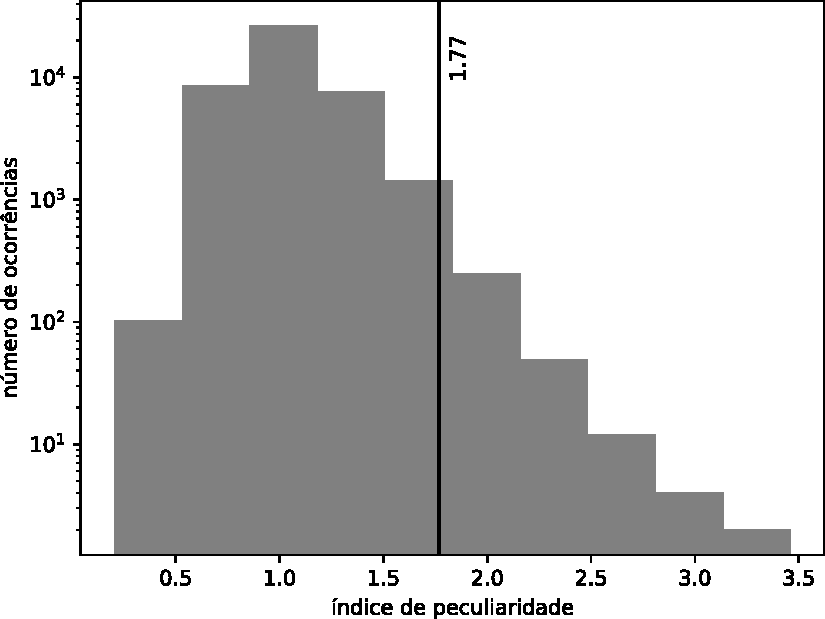
\includegraphics[width=0.5\textwidth]{peculiarity_histogram.pdf}
\caption{Histograma do índice de peculiaridade utilizando livros do Projeto Gutenberg como corpus.}
\label{fig-peculiarity_histogram}
\source{Elaboração própria.}
\end{figure}

O índice de peculiaridade pode ser utilizado como um bom indicativo de malformação de uma sequência de caracteres. 
A seguir, apresenta-se uma pequena lista de sequências encontradas no conjunto de livros extraídos do Projeto Gutenberg
e que possuem limiar de peculiaridade maior do que o limiar determinado:

\begin{lstlisting}[label=lst-peculiarwords]
armfeldt, bio, ciitzens, dulcineae, dwellingplaces, emunctae, expoliuntur, fayn, fortyfoot, funkyish, goerz, heytesbury, highminded, jommlin, milkjug, pistoia, pocketsful, rohgah, strikebreaker, twentythree, unpav, valentinavyczia, wiolent, wyman
\end{lstlisting}



% TYPO program on UNIX 
% "frequency of two-letter pairs (di- grams) and three-letter triples (tri- grams)"
% McMahon, L.E., Cherry, L.L., and Mor- ris, R. Statistical text processing. 
% Morris, R., and Cherry, L.L. Computer detection of typograhical errors. IEEE Trans. Professional Comm. PC-18, 1 (March 1975),
% "If a token contains several very rare digrams or trigrams, it is potentially misspelled."
% "The use of di- grams and trigrams to both detect probable spelling errors and indicate probable corrections
% has been one of the most popular techniques in the literature [5, 6, 16, 23, 24, 26, 32, 33, 42]."
% for each distinct token, an index of peculiarity is computed: [log(f(xy) - 1) + log (f(yz) - 1)]/2- log(f(xyz) - 1).
% (see Peterson pg 678)


% large dictionary may include rare, archaic, or obsolete words, and incorrectly spelled words

% two-level search strategy: first search in a small in-core table of most frequently used words,
% if not found, uses a larger dictionary
% (obs. memory is not a constraint anymore and hash table has constant time, regarless of its size)

% Damerau - 4 edits - 80 percent of all spelling errors 

% OCR - confusion matrix
%  characters that look alike... and pair edits linke rn and th and tn...
% sci-hub.tw/10.1145/2595188.2595200
% sci-hub.tw/10.1109/das.2016.44

% "A dictionary of 8,000 words would represent 90 percent of the words; 16,000 words would yield 95 percent."  (peterson)
% removing these affixes (an affix is either a suffix or a prefix) and storing only the root word, the dictionary can be reduced significantly


\section{Outras abordagens}\label{sec-outros}
As abordagens até então expostas neste trabalho utilizam características estatísticas da língua
para ordenar potenciais candidatos.
Há, contudo, outras informações
que podem ser incorporadas
às análises
a fim de auxiliar 
na organização e na definição dos
candidatos mais prováveis, a depender
do tipo de texto.
Por exemplo, se o corretor ortográfico atuar no pós-processamento
de um sistema de reconhecimento de caracteres (OCR, \textit{Optical Character Recognition}),
passa a ser importante considerar a proximidade ótica dos caracteres, de forma a corrigir erros 
gerados no processo de digitalização de documentos \cite{liu1991,tong1996,nagata1998,taghva2001,jrcacho2012}.
No caso em que se deseja corrigir erros
de datilografia, é intuitivo que se considere a proximidade das teclas
\cite{min1995,samuelsson2017} 
(ideia semelhante é utilizada pelo algoritmo de Needleman-Wunsch em bioinformática para alinhar proteínas
e nucleotídeos).
Ainda, se o objetivo é abarcar erros gerados pela falta de proficiência de indivíduos na tarefa de
soletrar palavras, pode-se considerar a vizinhança fonológica de sequências em uma língua \cite{avanco2014,pilan2018}.
Embora essas abordagens não sejam
tratadas neste texto, há uma família 
de corretores ortográficos que
abarcam tais temas disponíveis no repositório de um dos autores deste
artigo \cite{leolcaspell}.



%\begin{figure}[htbp]
% \centering
% \includegraphics[width=0.5\textwidth]{example-image-a}
% \caption{Imagem de teste.}
% \label{fig-img-a}
%\end{figure}

%\begin{table}[htbp]
%\centering
%\caption{Tabela de exemplo para o Texto Livre}\label{tab-exemplo}
%\begin{tabular}{cccc}
%\toprule
%  Dec  & Bin       & Octal & Hexa \\
%\midrule  
%  33   & 100001    &  41   & 21   \\
%\midrule
%  431  & 110101111 & 657   & 1AF  \\
%\bottomrule
%\end{tabular}
%\end{table}



\section{Resultados}
Apresentam-se, a seguir, os resultados 
da implementação do corretor
ortográfico proposto
por \textcite{norvig2007} aplicados
a um conjunto de arquivos de erros ortográficos de Birkbeck, criada por Roger Mitton e proveniente de diversas fontes reunidas no
Arquivo de Textos de Oxford (\textit{Oxford Text Archive}). Encontram-se entre eles os resultados de ditados para teste de ortografia e de erros em escrita livre,
grande parte deles escritos à mão. Os dados foram obtidos de crianças em idade escolar e de alunos universitários ou adultos letrados. Para que a análise
seja realizada, de início, verificam-se a acuracidade do corretor 
ortográfico no reconhecimento de palavras corretas ou incorretas
do ponto de vista ortográfico e os efeitos do emprego de regras para a
remoção dos afixos. Em sequência, verifica-se  a
efetividade das sugestões geradas pelo corretor.

Como salientado, o intuito de remover afixos é expandir
virtualmente o dicionário usado pelo corretor
ortográfico e, assim, diminuir a taxa de palavras indicadas
como ortograficamente erradas. Uma palavra não
encontrada no dicionário pode passar a ser quando se
remove dela os afixos, como demonstram
os resultados apresentados na \Cref{tbl-confusion}. Observa-se que, no
corpus em questão, há um acréscimo de, aproximadamente,
5,2\% de palavras corretas que são analisadas como
ortograficamente adequadas.
`\textit{Accessibility}', `\textit{choices}', `\textit{unequalled}', por exemplo, que até então
eram palavras desconhecidas para o corretor, passaram a ser consideradas
ortograficamente corretas após a remoção dos afixos. A incorporação
ocorreu porque as palavras `\textit{accessible}', `\textit{choice}' e `\textit{unequal}', respectivamente, 
encontram-se no dicionário e, portanto, promoveram a incorporação de vocábulos derivados
como palavras possíveis na língua. É interessante destacar que a percentagem
pode ser ainda maior se a língua em estudo tiver uma riqueza morfológica
maior do que o inglês.

\begin{table}[htpb]
\centering
\caption{Matriz de confusão do corretor ortográfico na tarefa de reconhecimento de palavras (ortografia correta e com erro ortográfico).}
\label{tbl-confusion}
\begin{subtable}{.5\linewidth}
    \centering
    \caption{Sem remoção de afixos.}
    \label{tbl-confusion-1}
    \begin{tabular}{ll|c|c|l}
    \cline{3-4}&    & \multicolumn{2}{c|}{categoria verdadeira}   &  \\  \cline{3-4} &   & correta & erro  & \\   \cline{1-4}
    \multicolumn{1}{|c|}{\parbox[t]{4mm}{\multirow{2}{*}{\rotatebox[]{90}{\centering corretor}}}}
      & \multicolumn{1}{c|}{\rotatebox[]{90}{\centering \ correta\ }}			& 430 & 14  &  \\ \cline{2-4}
    \multicolumn{1}{|c|}{} & \multicolumn{1}{c|}{\rotatebox[]{90}{\centering \ erro\ }} & 52  & 648 &  \\ \cline{1-4}
    \end{tabular}
\end{subtable}%
\begin{subtable}{.5\linewidth}
    \centering
    \caption{Com remoção de afixos.}
    \label{tbl-confusion-2}
    \begin{tabular}{ll|c|c|l}
    \cline{3-4}&    & \multicolumn{2}{c|}{categoria verdadeira}   &  \\  \cline{3-4} &   & correta & erro  & \\   \cline{1-4}
    \multicolumn{1}{|c|}{\parbox[t]{4mm}{\multirow{2}{*}{\rotatebox[]{90}{\centering corretor}}}}
      & \multicolumn{1}{c|}{\rotatebox[]{90}{\centering \ correta\ }}			& 455 & 55 &  \\ \cline{2-4}
    \multicolumn{1}{|c|}{} & \multicolumn{1}{c|}{\rotatebox[]{90}{\centering \ erro\ }} & 27 & 607 &  \\ \cline{1-4}
    \end{tabular}
\end{subtable}
\source{Elaboração própria.}
\end{table}

Observe, entretanto, que, assim como há um maior índice de acerto do corretor no
que se refere à inclusão de palavras corretas no banco de dados, há
também um aumento na quantidade de palavras que
contêm erros ortográficos que desacertadamente são consideradas corretas 
quando seus afixos são removidos, como exposto na \Cref{tbl-confusion}.
O número de palavras erradas que são analisadas pelo corretor como corretas
sobe de 14 para 55, levando a um acréscimo de 6,2\% de erros nessa
categoria. Ao terem seus sufixos removidos, sequências como `\textit{voteing}', `\textit{timeing}' e `\textit{lates}' passam a
ser interpretadas como palavras corretas, visto que `\textit{vote}', `\textit{time}' e `\textit{late}' são
palavras existentes e estão no dicionário. 

Embora, à primeira vista, a diferença entre o corretor sem remoção de afixo (\Cref{tbl-confusion-1}) e
com remoção de afixo (\Cref{tbl-confusion-2}) seja pequena, em uma análise de
300 amostras aleatórias do corpus em estudo, calculou-se o valor preditivo positivo, dado por $CE/(CC+CE)$,
e o valor preditivo negativo, dado por  $EC/(EC+EE)$,
onde CC, EC, EC e EE são os elementos da matriz de confusão, na ordem em que são apresentados na \Cref{tbl-confusion}.

A \Cref{fig-idx-300-tst} apresenta o histograma,
a partir do qual se verificou que a diferença entre os corretores é significativa.
A barra em preto vertical expressa os valores preditivos 
obtidos pela \Cref{tbl-confusion}, indicando valores
próximos à média das distribuições. 
Um corretor ortográfico que inclua processos de remoção de afixos traz,
portanto, ganhos significativos para
a identificação de vocábulos corretos,
ao custo de não identificar alguns vocábulos 
com possíveis erros ortográficos.

% precision or positive predictive value (PPV)
% tp/(tp+fp) = CC/(CC+CE) 

% negative predictive value (NPV) 
% fn/(fn+tn) = EC/(EC+EE)

\begin{figure}[h]
\centering
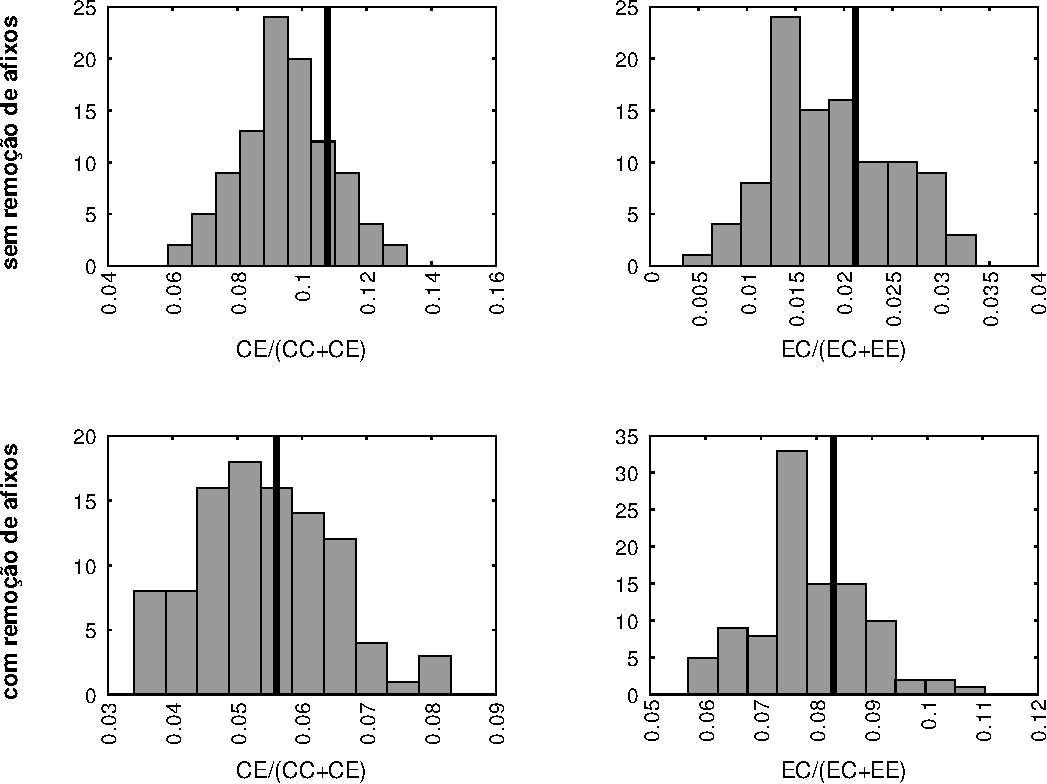
\includegraphics[width=0.75\textwidth]{hist_confmtx.pdf}
\caption{Resultado da distribuição dos valores preditivos positivo e negativo, gerados a partir de 300 amostras aleatórias. A barra preta vertical apresenta o valor obtido na \Cref{tbl-confusion}.}
\label{fig-idx-300-tst}
\source{Elaboração própria.}
\end{figure}

Ademais, é interessante destacar que o corretor ortográfico, apesar da
remoção dos afixos, continua classificando 
palavras reais, como `\textit{graphically}' e `\textit{unequivocally}' como ortograficamente
erradas. Destacam-se, para estes casos, duas imprecisões do corretor: a
ausência de recursividade no processo de afixação e a
limitação do corpus base para a formação do dicionário. O primeiro refere-se aos
processos de afixação que
ocorrem em sequência: `\textit{graphic}' $\rightarrow$ `\textit{graphical}' $\rightarrow$ `\textit{graphically}' e, em
alguns casos, com modificação no radical da palavra: `\textit{unequivocally}' $\rightarrow$
`\textit{unequivocal}' $\rightarrow$ `\textit{equivocal}' $\rightarrow$ `\textit{equivoque}'.  Perceba que a reaplicação
do processo de remoção dos afixos poderia ser eficiente para o primeiro 
exemplo, mas não para o segundo. Para este, faz-se necessária uma análise
morfofonológica mais refinada. Os exemplos descritos, ainda, evidenciam 
as limitações impostas por qualquer banco de dados, sendo, assim, importante
o uso de um dicionário ou de um corpus que seja, de fato, representativo da
língua.

No que se refere à efetividade das sugestões de candidatos para a
correção de palavras com erro ortográfico, observa-se, conforme exposto
na \Cref{tab-corate}, que a taxa de acerto cresce ao se aumentar o
número de candidatos.
Os candidatos são gerados pelas regras de mínima edição e ordenados
pelo número de edições e pela frequência 
de ocorrência no corpus das palavras geradas.
A diferença entre os valores preditivos negativos para os corretores,
com e sem remoção de afixos, é pequena, não impactando no
desempenho da correção.

\begin{table}[htbp]
\centering
\caption{Taxa de acerto na proposição de correção, em função do número de candidatos apresentados.}
\label{tab-corate}
\begin{tabular}{lllll}
\toprule
remoção de sufixo & \multicolumn{4}{l}{número de candidatos} \\
                & 1        & 3        & 5        & 7       \\
\midrule
sem remoção     & 0.702   & 0.798   & 0.816   & 0.822  \\
com remoção     & 0.702   & 0.798   & 0.816   & 0.822  \\
\bottomrule
\end{tabular}
\source{Elaboração própria.}
\end{table}

%\textbf{Leo, sugiro tirar essa última parte, pois os resultados só são apresentados e, para fazer uma discussão, precisaríamos dos valores também com a remoção dos afixos. Deixaria para explorar, então, em outros trabalhos, se for o caso.}

Roger Mitton ainda disponibiliza em sua página pessoal\footnote{\url{https://www.dcs.bbk.ac.uk/{\~}ROGER/corpora.html}} outras bases
de dados que serão aqui utilizadas: Holbrook (inclui erros ortográficos produzidos à mão por crianças no último ano escolar),
\textit{Aspell} (contém os dados coletados por Kevin Atkinson para testar o \textit{Aspell}) e Wikipedia (contém erros de ortografia cometidos
pelos contribuidores da Wikipedia). As duas últimas bases de dados, portanto, são obtidas de textos datilografados.
É importante verificar a forma com que
cada um dos dados foram obtidos, pois podem representar diferentes tipos de
erros.

%\begin{minipage}
\begin{table}[htbp]
\centering
\caption{Bases de dados utilizadas para os testes de performance dos corretores ortográficos.}\label{tab-data}
\begin{tabular}{cccc}
\toprule
  nome      & erros ortográficos    & palavras  & forma   \\
\midrule  
  Birkbeck  & 36.133                & 6.136     & escrito à mão$^{*}$\\
\midrule
  Holbrook  & 1791                  & 1200      & escrito à mão \\
\midrule
  Aspell    & 531                   & 450       & datilografado \\
\midrule
  Wikipedia & 2.455                 & 1.922     & datilografado \\
\bottomrule
\end{tabular}
    \vspace{1ex}

    { \hspace{18em} \footnotesize $^{*}$ em grande parte \par}

\source{Elaboração própria.}
\end{table}
%\end{minipage}



\begin{table}[htpb]
\centering
\caption{Matriz de confusão do corretor ortográfico na tarefa de reconhecimento de palavras sem a remoção de afixos.}
\label{tbl-confusion-all}
\begin{subtable}{.5\linewidth}
    \centering
    \caption{Birkbeck.}
    \label{tbl-confusion-all-1}
    \begin{tabular}{ll|c|c|l}
    \cline{3-4}&    & \multicolumn{2}{c|}{categoria verdadeira}   &  \\  \cline{3-4} &   & correta & erro  & \\   \cline{1-4}
    \multicolumn{1}{|c|}{\parbox[t]{4mm}{\multirow{2}{*}{\rotatebox[]{90}{\centering corretor}}}}
      & \multicolumn{1}{c|}{\rotatebox[]{90}{\centering \ correta\ }}			& 5142 & 3129   &  \\ \cline{2-4}
    \multicolumn{1}{|c|}{} & \multicolumn{1}{c|}{\rotatebox[]{90}{\centering \ erro\ }} & 824 & 32712 &  \\ \cline{1-4}
    \end{tabular}
\end{subtable}%
\begin{subtable}{.5\linewidth}
    \centering
    \caption{Holbrook.}
    \label{tbl-confusion-all-2}
    \begin{tabular}{ll|c|c|l}
    \cline{3-4}&    & \multicolumn{2}{c|}{categoria verdadeira}   &  \\  \cline{3-4} &   & correta & erro  & \\   \cline{1-4}
    \multicolumn{1}{|c|}{\parbox[t]{4mm}{\multirow{2}{*}{\rotatebox[]{90}{\centering corretor}}}}
      & \multicolumn{1}{c|}{\rotatebox[]{90}{\centering \ correta\ }}			& 894 & 477 &  \\ \cline{2-4}
    \multicolumn{1}{|c|}{} & \multicolumn{1}{c|}{\rotatebox[]{90}{\centering \ erro\ }} & 224 & 1283 &  \\ \cline{1-4}
    \end{tabular}
\end{subtable}

    \vspace{3ex}

\begin{subtable}{.5\linewidth}
    \centering
    \caption{Aspell.}
    \label{tbl-confusion-all-3}
    \begin{tabular}{ll|c|c|l}
    \cline{3-4}&    & \multicolumn{2}{c|}{categoria verdadeira}   &  \\  \cline{3-4} &   & correta & erro  & \\   \cline{1-4}
    \multicolumn{1}{|c|}{\parbox[t]{4mm}{\multirow{2}{*}{\rotatebox[]{90}{\centering corretor}}}}
      & \multicolumn{1}{c|}{\rotatebox[]{90}{\centering \ correta\ }}			& 337 & 15  &  \\ \cline{2-4}
    \multicolumn{1}{|c|}{} & \multicolumn{1}{c|}{\rotatebox[]{90}{\centering \ erro\ }} & 112  & 515  &  \\ \cline{1-4}
    \end{tabular}
\end{subtable}%
\begin{subtable}{.5\linewidth}
    \centering
    \caption{Wikipedia.}
    \label{tbl-confusion-all-4}
    \begin{tabular}{ll|c|c|l}
    \cline{3-4}&    & \multicolumn{2}{c|}{categoria verdadeira}   &  \\  \cline{3-4} &   & correta & erro  & \\   \cline{1-4}
    \multicolumn{1}{|c|}{\parbox[t]{4mm}{\multirow{2}{*}{\rotatebox[]{90}{\centering corretor}}}}
      & \multicolumn{1}{c|}{\rotatebox[]{90}{\centering \ correta\ }}			& 1395 & 12 &  \\ \cline{2-4}
    \multicolumn{1}{|c|}{} & \multicolumn{1}{c|}{\rotatebox[]{90}{\centering \ erro\ }} & 516 & 2443  &  \\ \cline{1-4}
    \end{tabular}
\end{subtable}
\source{Elaboração própria.}
\end{table}


\begin{table}[htbp]
\centering
\caption{Taxa de acerto na proposição de correção, em função do número de candidatos apresentados.}
\label{tab-corate-all}
\begin{tabular}{lllll}
\toprule
base de dados & \multicolumn{4}{l}{número de candidatos} \\
                & 1        & 3        & 5        & 7       \\
\midrule
Birkbeck   & 0.315 & 0.377 & 0.391 & 0.397 \\
Holbrook   & 0.260 & 0.322 & 0.341 & 0.353 \\
Aspell	   & 0.433 & 0.533 & 0.546 & 0.554 \\
Wikipedia  & 0.607 & 0.692 & 0.702 & 0.705 \\
\bottomrule
\end{tabular}
\source{Elaboração própria.}
\end{table}



% bases de dados dos testes
% testes e resultados

% remover afixos pode resolver alguns problemas e criar novos
% Usando a mesmas base de dados utilizada por Norvig.
% O intuito de remover afixos é diminuir a taxa de falso negativo,
% pois, ao remover um afixo, podemos encontrar a palavra raiz no dicionário 
% em que a palavra derivada (pela adição de afixo) não estava presente.
% As seguintes palavras, por exemplo, passam a ser consideradas corretas
% pelo verificador ortográfico apenas após remover os afixos: 'accessibility',
% 'accessing', 'generated', 'queries', dentre outras.
% Por outro lado, palavras com erros ortográficos podem ser erroneamente 
% consideradas corretas quando remove-se delas afixos. 
% Com exemplo, temos que as palavras: 'voteing', 'timeing', 'lates' encontram 
% suas versões sem afixo 'vote', 'time', 'late' no dicionário,
% aumentando assim a taxas de falso positivo.

% RESULTADOS norvig1 e norvig2 datasets:
%
% resultados (removendo afixos) - 482 samples
% 444 true positives, 38 false positives
% 635 true negatives, 27 false negatives
% 2.564537286758423 sec
%
% resultados (sem remover afixos) - 482 samples
% 430 true positives, 52 false positives
% 648 true negatives, 14 false negatives
% 0.4725186824798584 sec

% grep "False is not true" spell_unittest_20200626-140329.log | cut -d "=" -f2 | sed 's/^ *//g' > /tmp/false-negatives-suffix-removal.txt 
% grep "False is not true" spell_unittest_20200626-140728.log | cut -d "=" -f2 | sed 's/^ *//g' > /tmp/false-negatives.txt
% diff <(sort /tmp/false-negatives-suffix-removal.txt) <(sort /tmp/false-negatives.txt)
% accessibility, accessing, analysed, apologised, arrangeing, assessing, choices, conditioning
% embellishing, generated, guidelines, queries, techniques, unequalled
% >>> 'planed' in myspell.WORDS
% True 
% >>> 'accessibility' in myspell.WORDS                                                             
% False
% >>> 'accessible' in myspell.WORDS                                                                
% True
% >>> 'choices' in myspell.WORDS                                                                   
% False
% >>> 'choice' in myspell.WORDS                                                                    
% True
% >>> 'unequalled' in myspell.WORDS
% False
% >>> 'unequal' in myspell.WORDS
% True
% >>> 'equal' in myspell.WORDS
% True



%%%% sugestion test restuls
% test_suggestions ran in: 40.917372941970825 sec
% test: test_suggestions >>> TestSpell has corrected 468 from 662 spelling errors (70.7% correction rate)
%
% list of real word errors found:
% 'contented', 'wonted', 'planed', 'humor', 'et', 'equaled', 'advice', 'where',
% 'latter', 'unequaled'

% norvig1,2
% suffix remove
% test suggestions
% python3 -m unittest tests.test_spellclasses.TestSpell.test_suggestions
% spell_unittest_20200626-134431.log
% test isknown
% python3 -m unittest tests.test_spellclasses.TestSpell.test_isknown
% spell_unittest_20200626-140329.log

% norvig1,2
% NO suffix removal
% test suggestions
% python3 -m unittest tests.test_spellclasses.TestSpell.test_suggestions
% spell_unittest_20200626-140553.log
% test isknown
% python3 -m unittest tests.test_spellclasses.TestSpell.test_isknown 
% spell_unittest_20200626-140728.log

%%%% CORRECTION RATE TEST
% num candidates	1	3	5	7	
% NO suffix removal	70.7%	79.9%	81.7%	82.2%
% SUFFIX removal	70.7%	79.8%	81.7%	82.2%

\section{Conclusão}
O presente trabalho apresentou uma revisão sobre o desenvolvimento de corretores ortográficos, especificando
as estratégias e as ferramentas
propostas por cada um deles.
Mostrou-se, a partir de algumas
ideias expostas por \textcite{norvig2007,robbins2005}, 
como é possível
criar um corretor ortográfico simples e eficiente, o qual pode ser facilmente
adaptado para diversas línguas. 

Em resumo, para realizar a tarefa de detecção de erro, verificou-se se a sequência de busca se
encontrava no léxico gerado por um
grande corpus. Caso não fosse encontrada, observava-se se havia
nela a presença de afixo. Em caso afirmativo, aplicavam-se regras para
remoção de afixos e buscava-se
encontrar o radical da palavra no
dicionário. Constatou-se que os corretores, com
e sem remoção de afixo, apresentam resultados
significativamente distintos, porém, 
o desempenho dos corretores na tarefa de corrigir
erros ortográficos é essencialmente a mesma. 
Conforme previamente observado,
a remoção de afixos, sem levar em consideração os aspectos gramaticais,
costuma acarretar a aceitação
de palavras grafadas de
forma errada, não 
sendo, portanto, uma boa estratégia de
correção ortográfica.
Como abordagem alternativa,
\textcite{elliott1988} propôs a utilização de classes
de equivalência
de afixos para obter melhores resultados.

Embora os erros de palavras reais sejam
relevantes, é importante ressaltar que o exemplo de corretor ortográfico proposto por \textcite{norvig2007} não visa os
corrigir, nem os erros gerados pela
inserção nem pelo apagamento de espaços
em branco em/entre palavras.
Segundo \textcite{verberne2002}, os erros de palavra real
compreendem de 25 a 40\% dos erros encontrados \cite{wing1980,mitton1987,young1991} e, 
segundo \textcite{kukich1992b}, os erros
gerados pela inserção ou pelo apagamento
de espaços abarcam cerca de 15\%.
Além disso, observou-se, no presente
trabalho e em \textcite{kukich1992},
que corretores ortográficos
de palavras isoladas podem corrigir, em geral, aproximadamente, 78\% dos erros ortográficos,
desde que não sejam erros de palavra real.
É preciso lembrar que, para gerar candidatos para corrigir os erros ortográficos, este trabalho utilizou 
operações de simples edição:
adição, remoção, substituição e transposição de caracteres. Nele, a
distância de edição e a frequência 
são utilizadas para ordenar e determinar quais são os melhores candidatos.
Os resultados alcançaram uma taxa de
70\% de êxito na correção e de,
aproximadamente, 82\%
na exposição da palavra correta
dentre os 5 primeiros candidatos.
Não é possível afirmar se existe um limite para a performance de um corretor ortográfico de palavras isoladas,
como o que foi apresentado neste trabalho. Entretanto, seres humanos desempenhando a mesma tarefa
alcançam em média uma taxa de acerto na correção de 74\% \cite{kukich1992}, o
que indica uma boa performance dos 
corretores aqui apresentados. 


% "25% to 40% of all errors are real-word errors" (Verberne 2002)
% "The performance of the spell checking application varies with lexicon size and the
% characteristics of the test set. Kukich (1992b) found that approximately 78% of
% non-word errors could be corrected by isolated-word correction techniques in general."
% Mitton (1987) found that 40%
% of all 4218 errors were real-word errors. Young, Eastman and Oakman (1991) found a real-word
% spelling error rate of 25%. Wing and Baddeley (1980) found that 30% of the errors were real-
% word errors. The percentage found by Peterson (16%) is much lower than the percentages found
% by others. This is because Peterson only considered errors resulting from single-error
% misspellings and the other studies also addressed errors resulting from more than one character
% transformation. 

%%% Verificar se o tamanho do corpus influencia.


%"Elliott [1988] describes in a memo on an improved morphological-processing component for 
%the Unix spell program, simple affix-stripping methods often lead to false acceptances,
%such as 'adviseed' or 'disclam', when affixes are stripped with no regard to grammar.
%Elliott provides an efficient solution based on creating affix equivalence classes that are
%motivated by spelling similarities." (Kukich, 1992)

Ressalta-se, por fim, que o corretor 
ortográfico foi escrito em Python, usando orientação a objetos,
tendo em vista que essa abordagem 
permite o reaproveitamento do código na elaboração de novos corretores ortográficos que considerem, por
exemplo, novas formas de identificar erros, gerar candidatos e ordená-los conforme
alguma métrica qualquer. Com a utilização de classes, é possível,
inclusive, criar corretores ortográficos
derivados de diferentes corretores, por
meio de múltiplas estratégias e de
métricas que geram 
e ranqueiam candidatos. Ademais,
o \textit{framework} criado para testar os corretores ortográficos poderá também
ser prontamente 
aplicado a novos corretores. Desta forma, torna-se fácil gerar testes e estabelecer comparações entre
diferentes abordagens.

Todos os códigos estão disponíveis no repositório no Github \cite{leolcaspell}, inclusive novos corretores que estão sendo
desenvolvidos pelo autor.


\printbibliography\label{sec-bib}
% if the text is not in Portuguese, it might be necessary to use the code below instead to print the correct ABNT abbreviations [s.n.], [s.l.] 
%\begin{portuguese}
%\printbibliography[title={Bibliography}]
%\end{portuguese}


\end{document}
